\chapter{Output}

This chapter describes the functional outputs of the Aether Co-Pilot system across its various modules. Due to the interactive nature of the application, the outputs are presented as categorized screenshots of the user interface during active sessions.

\section{admin login}
The admin login screen restricts access to system metrics. Only designated personnel mapped to specific roles in Firebase can successfully authenticate via Clerk.
\begin{figure}[!ht]
\centering
% \includegraphics[width=0.9\textwidth]{images/admin_login.png}
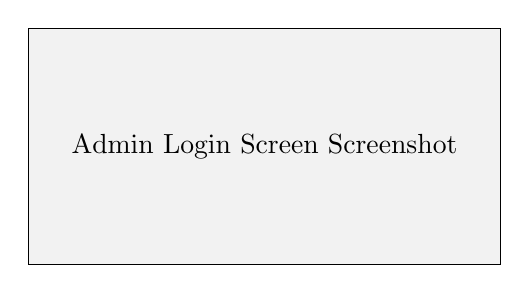
\begin{tikzpicture}
  \node[draw, rectangle, minimum width=6cm, minimum height=3cm, align=center, fill=gray!10] {Admin Login Screen Screenshot};
\end{tikzpicture}
\caption{Admin Login Portal}
\end{figure}

\section{admin dashboard}
The admin dashboard provides a holistic view. It includes graphs for API latency tracking (Gemini metrics) and memory storage utilization limits across the platform.
\begin{figure}[!ht]
\centering
% \includegraphics[width=0.9\textwidth]{images/admin_dash.png}
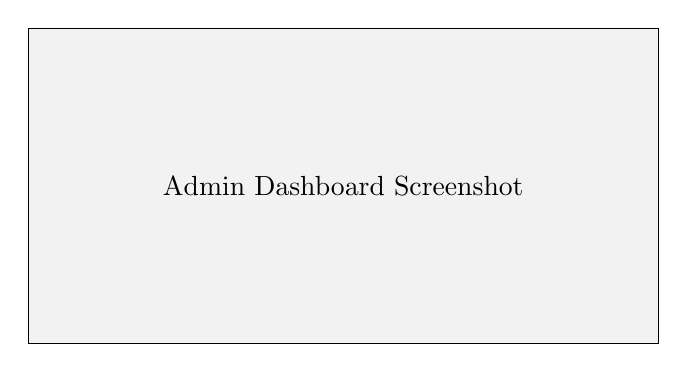
\begin{tikzpicture}
  \node[draw, rectangle, minimum width=8cm, minimum height=4cm, align=center, fill=gray!10] {Admin Dashboard Screenshot};
\end{tikzpicture}
\caption{Admin Dashboard View}
\end{figure}

\section{user registration}
The user registration process captures newly enrolled students and adds them into the secure Firestore sandbox, issuing an encryption key specifically tethered to their User ID.
\begin{figure}[!ht]
\centering
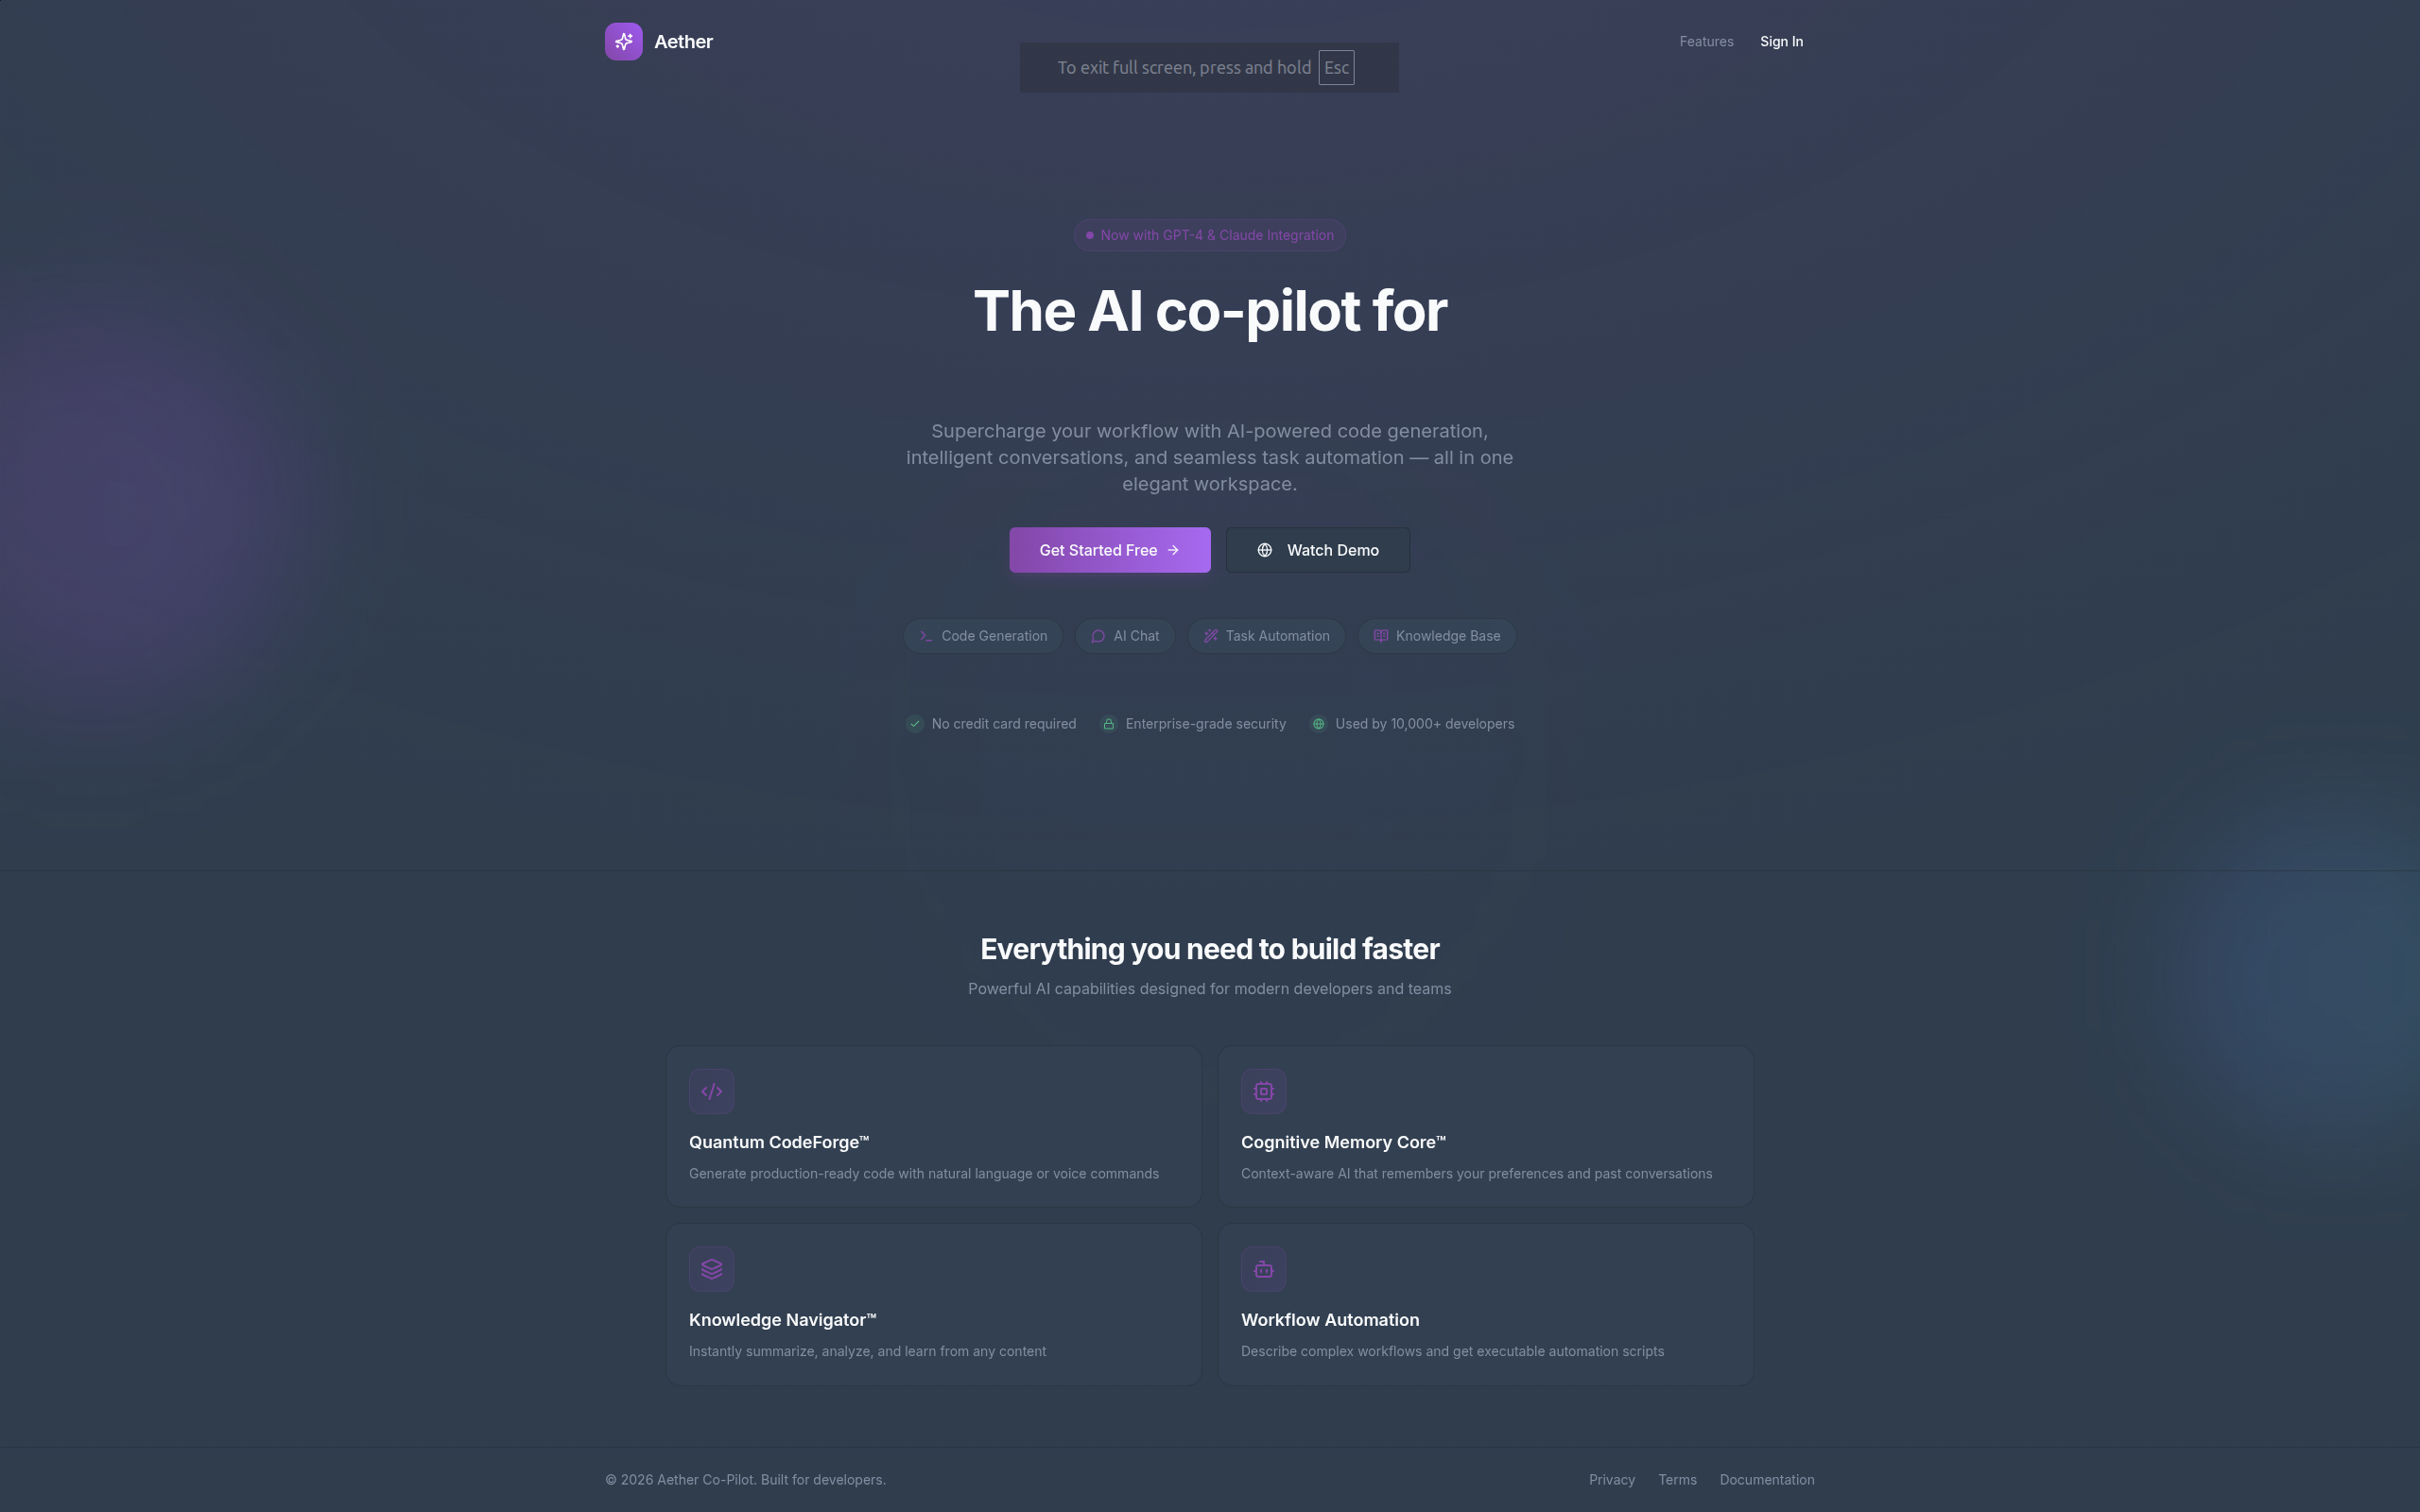
\includegraphics[width=0.9\textwidth]{images/Landing.png}
\caption{The Hero Interface \& Registration Trigger}
\end{figure}

\section{user login}
The user login flow is a seamless Modal triggered over the main app context. It supports social logins, bypassing manual entry.
\begin{figure}[!ht]
\centering
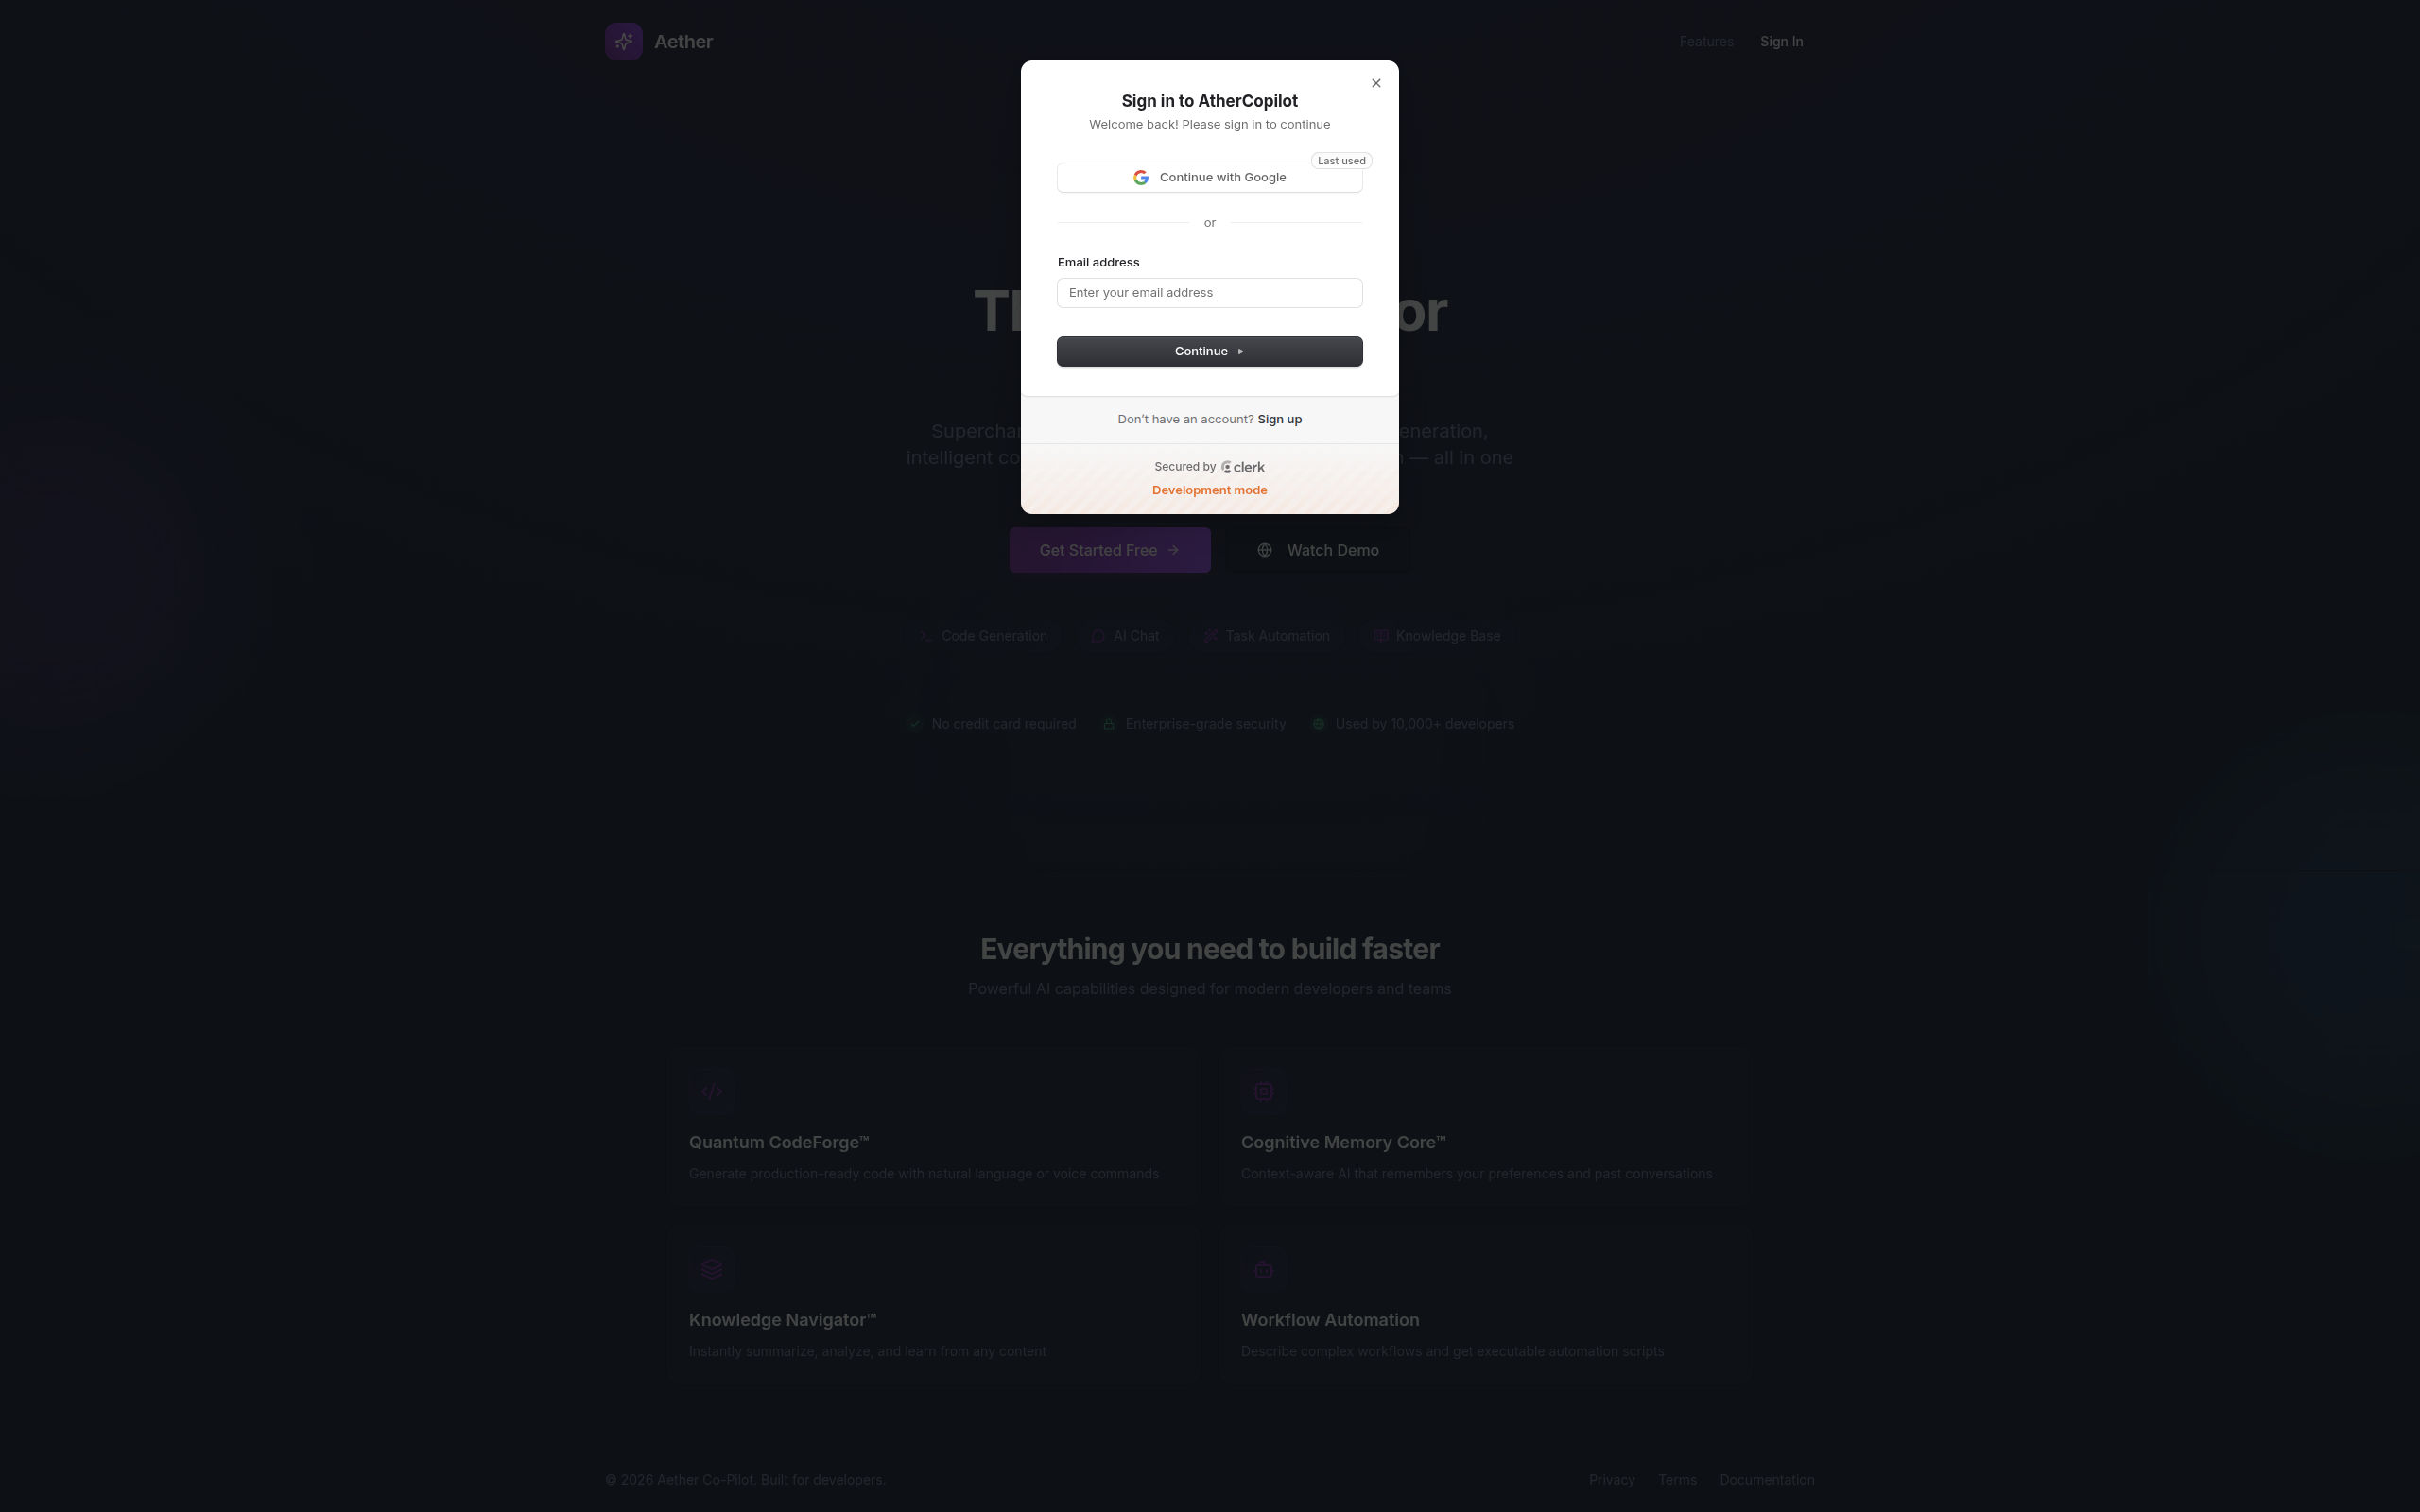
\includegraphics[width=0.9\textwidth]{images/Login.png}
\caption{Clerk Auth Modal for User Login}
\end{figure}

\section{profile list}
The profile management list allows users to view their active workspaces, subscription tier limits, and toggle application-wide dark or light mode.
\begin{figure}[!ht]
\centering
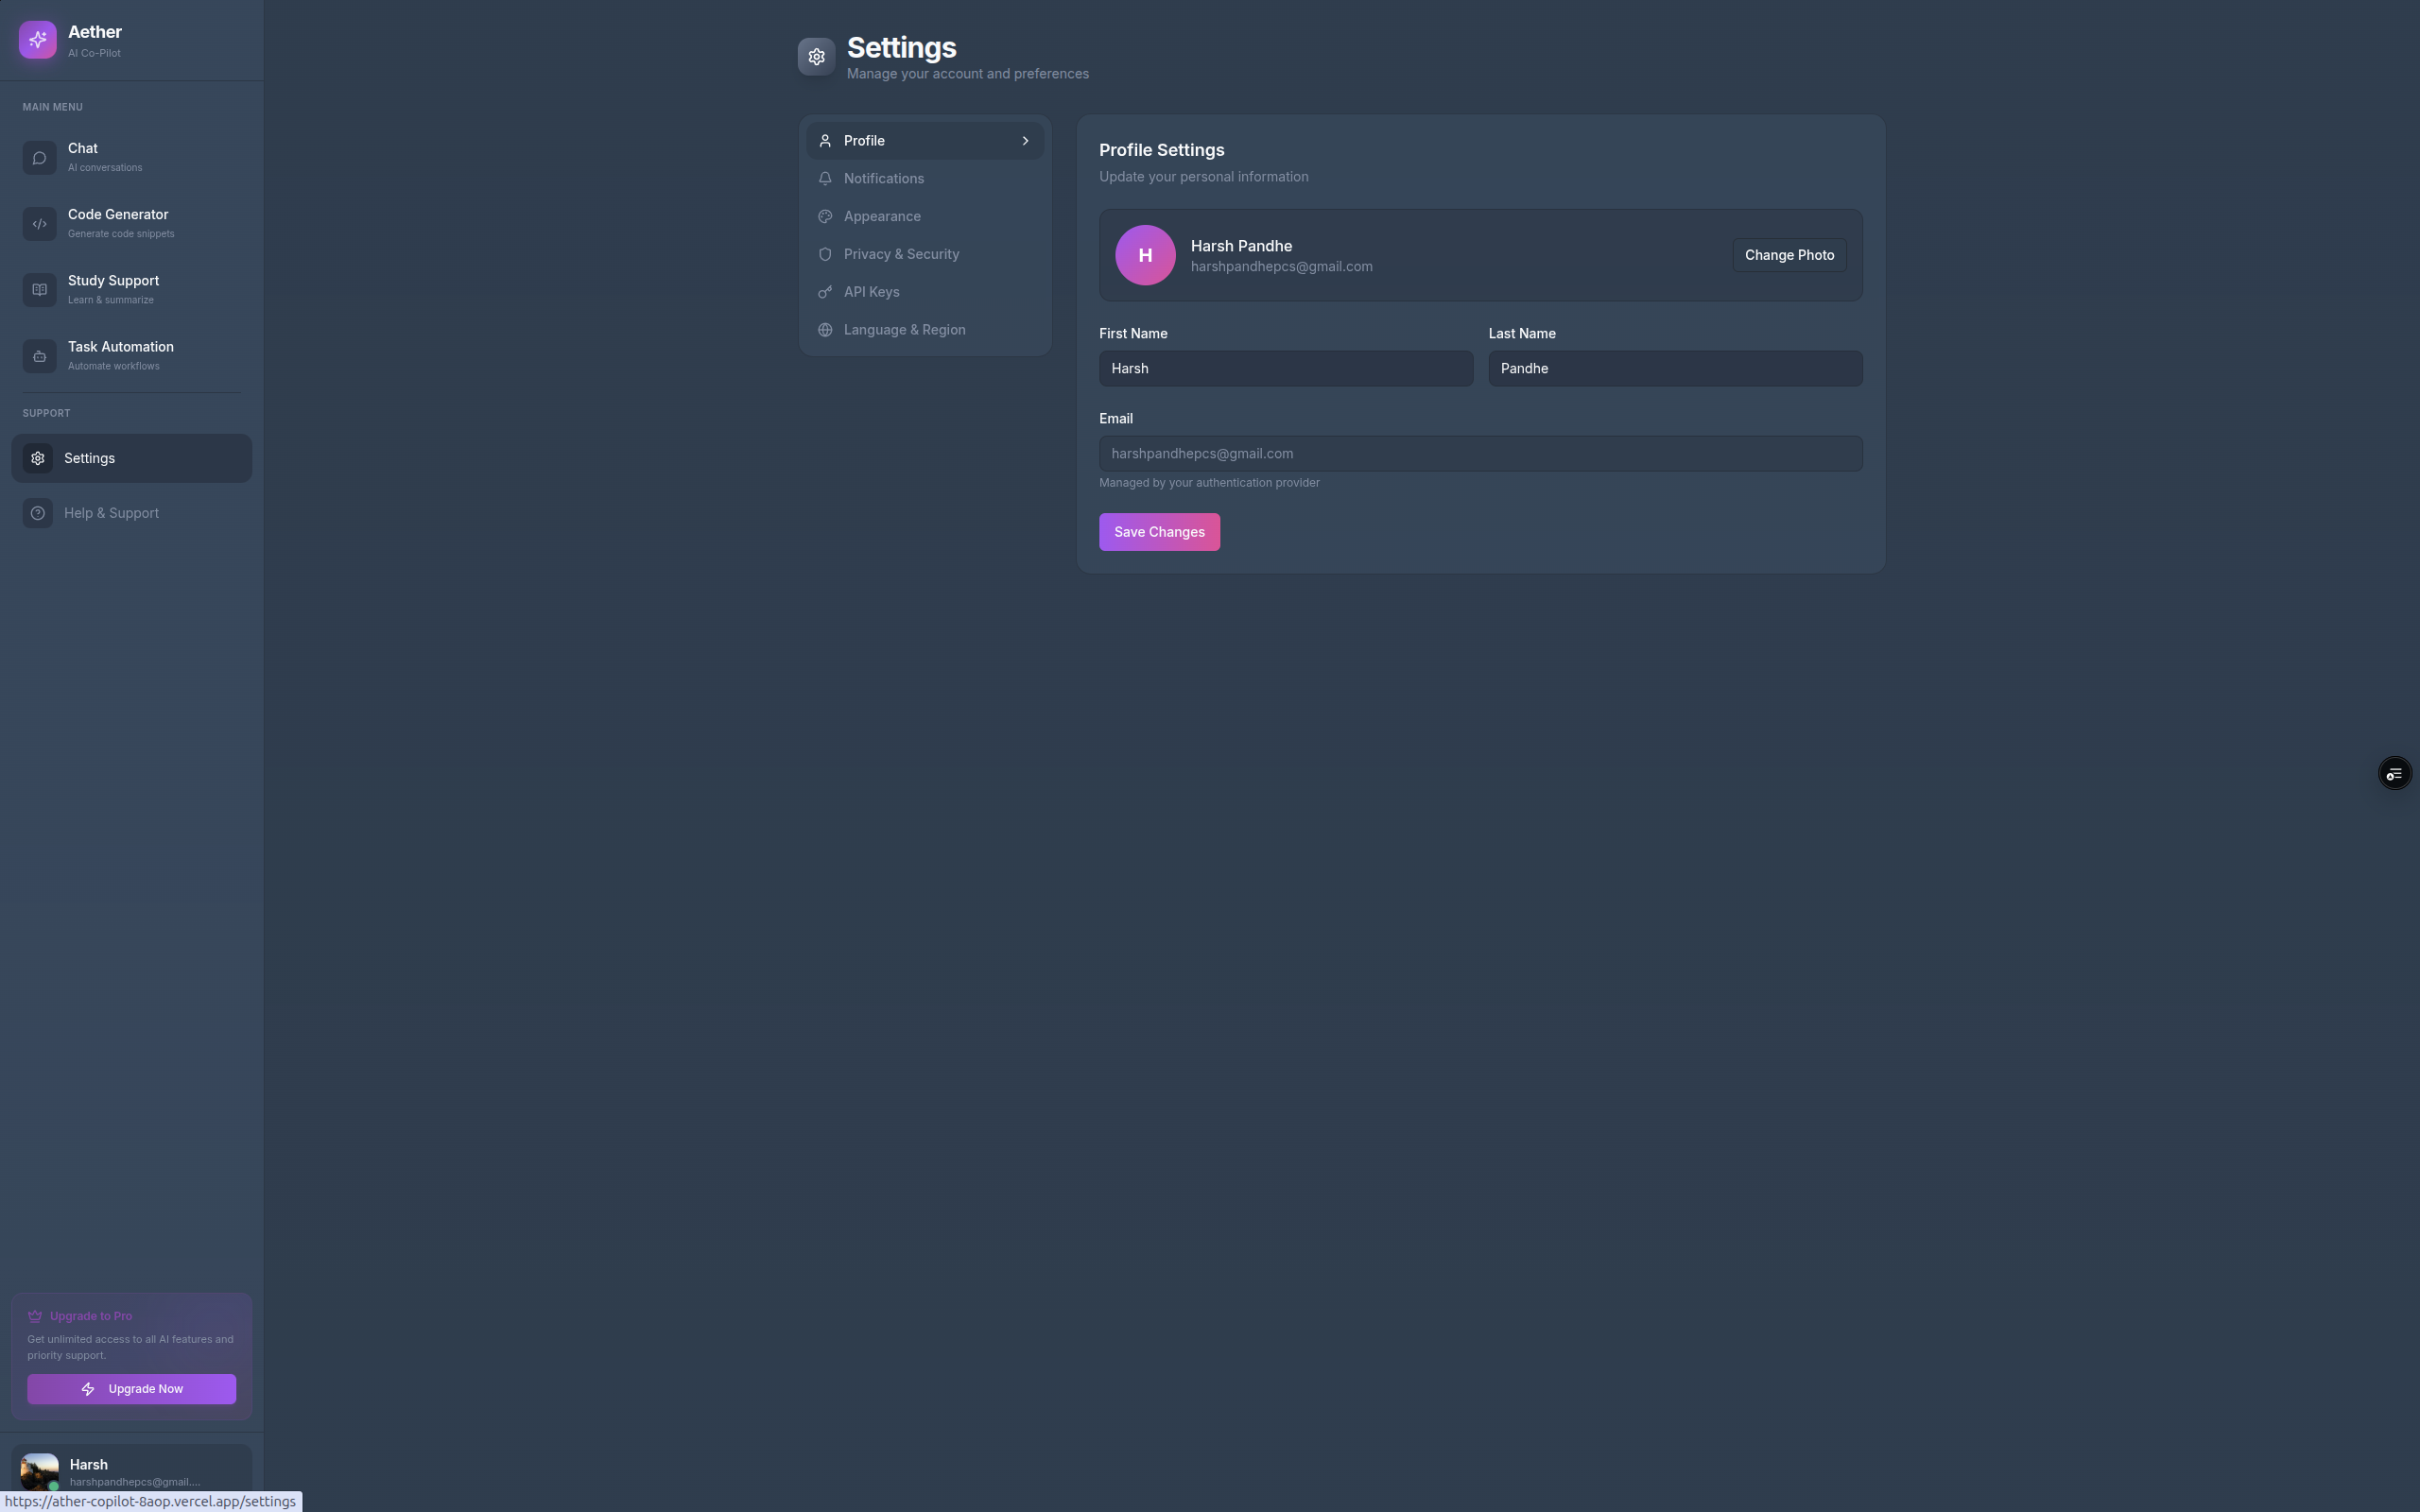
\includegraphics[width=0.9\textwidth]{images/Settings.png}
\caption{User Settings and Profile View}
\end{figure}

\section{Task automation}
The task automation module translates a natural language snippet into an executable Bash script for the local operating system.
\begin{figure}[!ht]
\centering
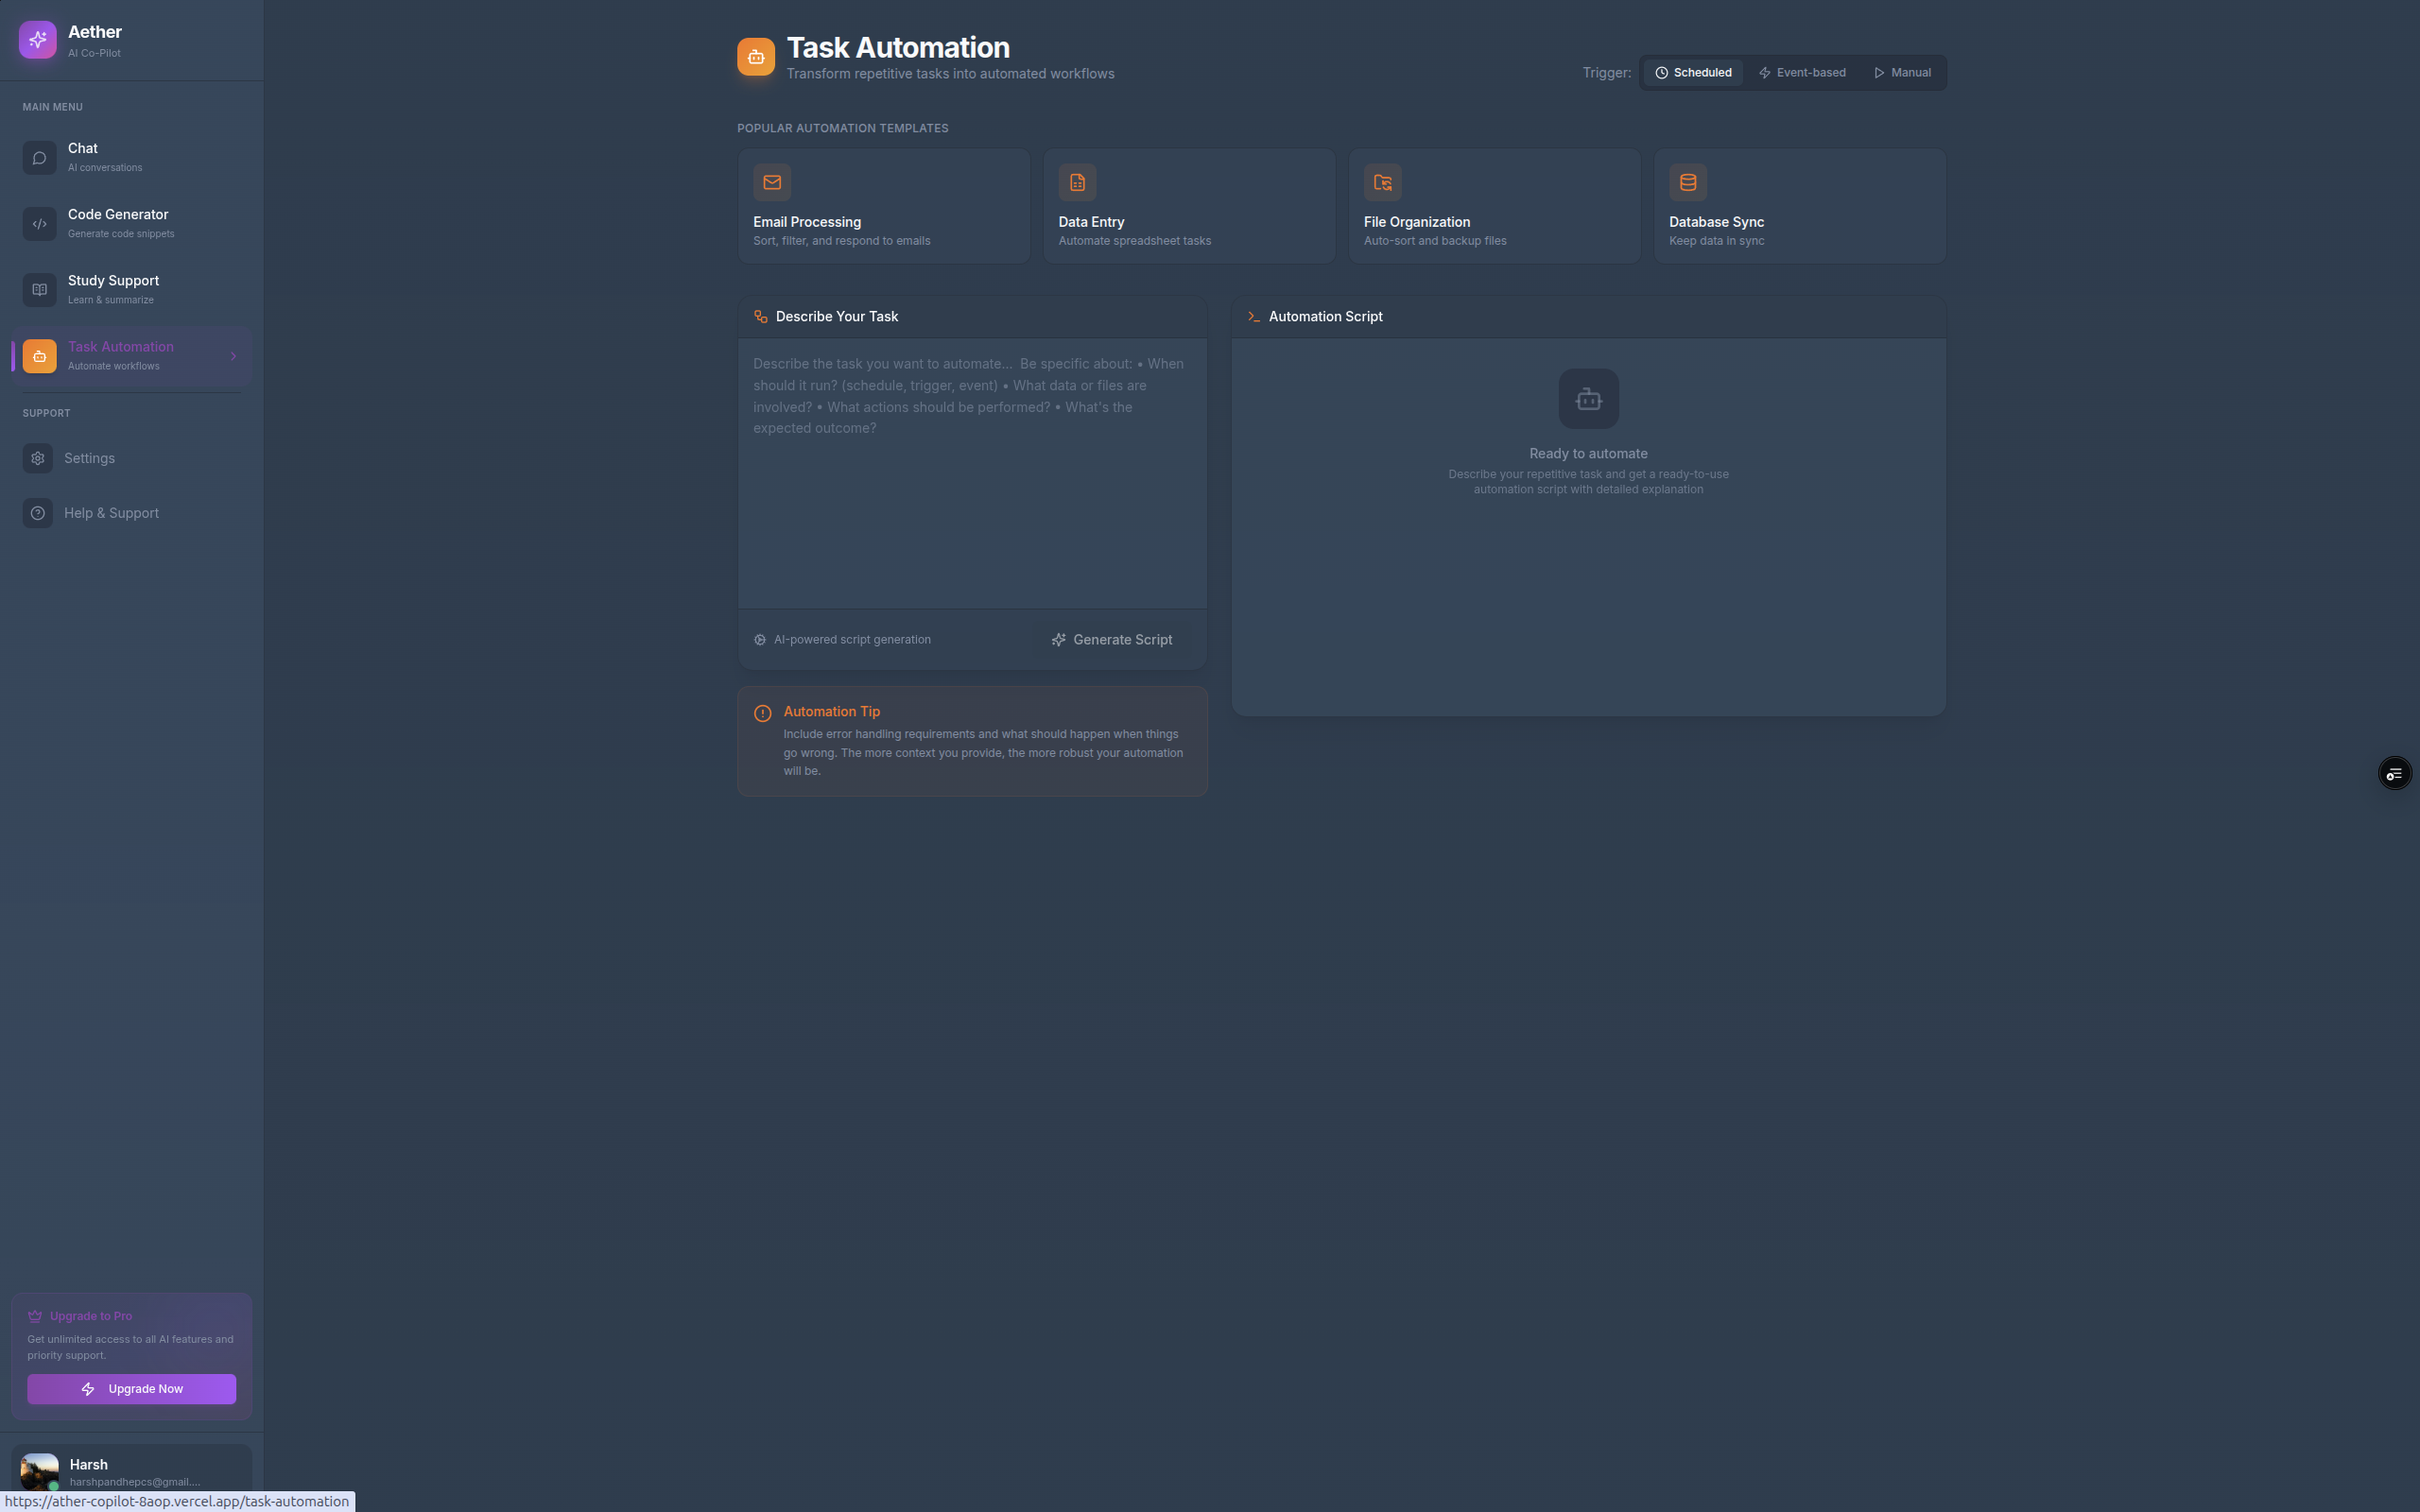
\includegraphics[width=0.9\textwidth]{images/Task.png}
\caption{Task Automation Engine Output}
\end{figure}

\section{Code generator}
Quantum CodeForge generates live code blocks from either text inputs or voice transcription prompts directly into the user interface.
\begin{figure}[!ht]
\centering
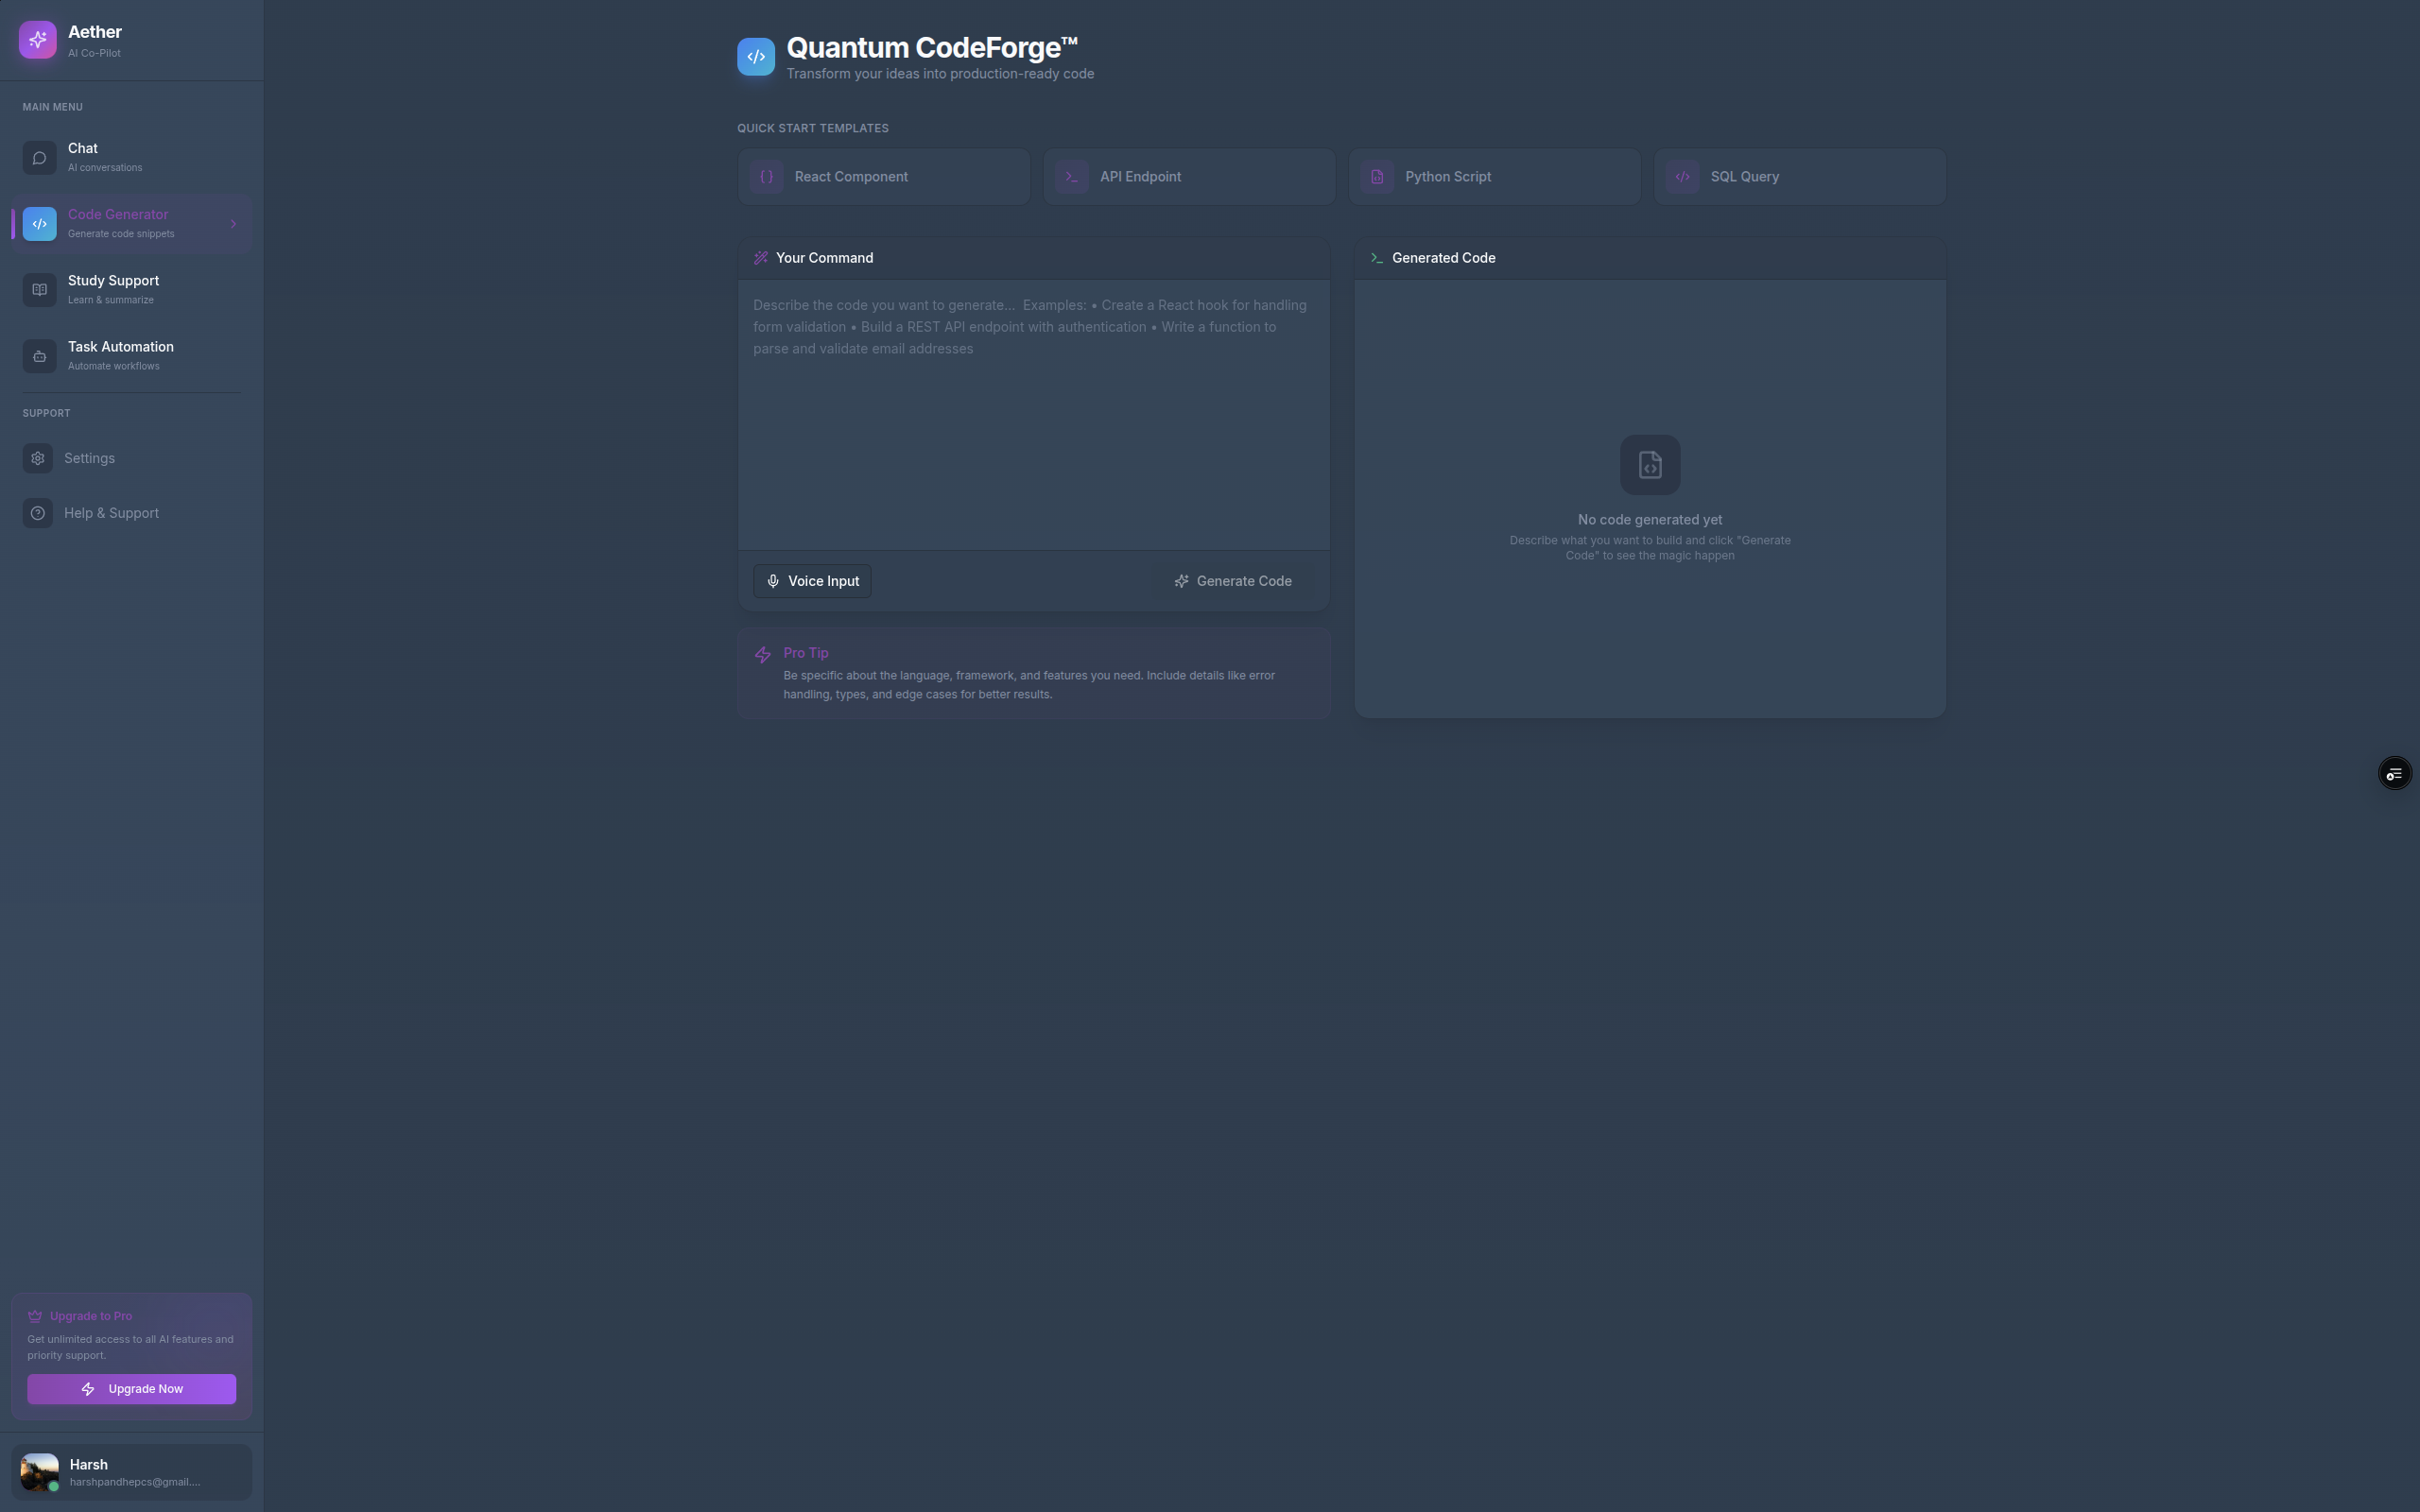
\includegraphics[width=0.9\textwidth]{images/Code.png}
\caption{Quantum CodeForge: Code Generation block}
\end{figure}

\newpage
